\skriptsection{Digitale Uebermittlung analoger Signale}{90}

%\subsection{PCM - Pulse Code Modulation}
\begin{center}
	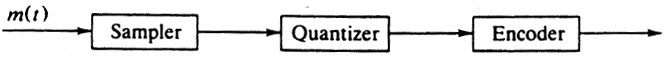
\includegraphics[width=10cm]{../NaT1/bilder/dig_pcm_blockdiagramm.png}
\end{center}
\begin{enumerate}
  \item Abtastung(Sampler): Zeitdiskretisierung 
  \item Quantisierung(Quantizer): Amplitudendiskretisierung
  \item Encoder(Codierung)
\end{enumerate}

Einige Vorteile der Digitalisierung: $\approx$ 100\% Störungsfrei, Algorithem einfach auf Signal
anwendbar, Verschlüsselung leicht gemacht.\\

\hrule
\skriptsubsection{Abtastung (Sampling)}{91-5.4}
Ein ideale Abtastung besteht theoretisch aus einer periodischen Abfolge von Dirac-Pulsen
$\delta_{T_S}$ mit dem Abstand $T_s = \frac{1}{f_s}$. Dieses Spektrum erhält man mittels der
Fourier-Reihe. \\ 
%$$ c_n = \frac{1}{T} \int\limits_{-T/2}^{T/2} \delta_{T_S}(t) e^{-j n \omega n t} dt = 
%\frac{1}{T} \quad \Rightarrow \quad X(j \omega) = \sum\limits_{n = -\infty}^{+\infty} c_n
%\delta(\omega - n \omega_0) \qquad 
$$ \delta_{T_S}(t) = \sum\limits_{n=-\infty}^{+\infty} \delta(t-nT_S) \laplace 
\omega_S \delta_{\omega_S} (j \omega) = 
\omega_S \sum\limits_{n=-\infty}^{+\infty} \delta(\omega - n \omega_S)$$
	\begin{center}
		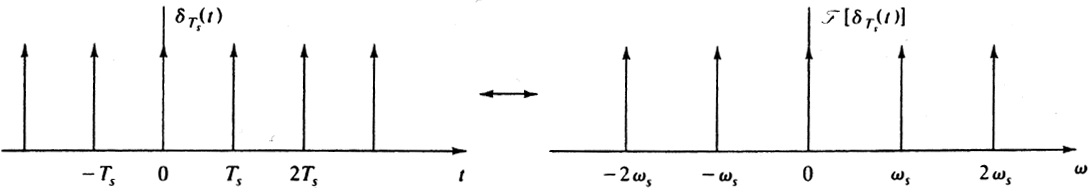
\includegraphics[width=10cm]{../NaT1/bilder/dig_sampler_ideal.png}
	\end{center}

\subsubsection{Abtasttheorem - Nyquist Theorem}
Ein Nachrichtensignal muss mind. mit dem Doppelten seiner Eigenfrequenz abgetastet werden. \\
Ansonsten können sich die Signale im Spektralbereich überlappen.  Um dies zu verhindern wird ein
sogenannter \textbf{Anti-Aliasing Filter} der Abtastung vorgeschaltet.\\
\begin{minipage}[t][2.7cm][c]{8cm}
$ f_s \geq 2 f_M $ \\
$ f_N = 2 \cdot B_M $ \\
$ f_{Nyq} = \frac{f_s}{2}$ \\
$ T_N = \frac{1}{2\cdot B_M} = \frac{1}{f_N} $

\end{minipage}
\begin{minipage}[t][2.7cm][c]{10cm}
	$f_s$ Samplingfrequenz, $[f_s] = Hz$ \\
	$f_M$ Nachrichtenfrequenz, $[f_M] = Hz$ \\
	$B_M$ Nachrichtenbandbreite, $[B_M] = Hz$ \\
	$f_N$ Nyquistrate, $[f_N] = Hz$ \\
	$f_{Nyq}$ Nyquistfrequenz, $[f_{Nyq}] = Hz$ \\
	$T_N$ Nyquistintervall, $[T_N] = s$ \\	
\end{minipage}

Handelt es sich bei dem Nachrichtensignal um ein \textbf{Bandpasssignal}, so kann mit einer noch
kleiner Samplingfrequenz abgetastet werden, dies nennt man \textbf{Subsampling}. \\
Vorgehen: 1. Alle möglichen $n$ bestimmen (ganzzahlig). 2. Alle möglichen Frequenzintervalle für
$f_s$ bestimmen.

\begin{minipage}[t][2cm][c]{10cm}
$$ 1 \leq n \leq \frac{f_u}{f_u - f_l} $$
$$ \frac{2 \cdot f_u}{n} \leq f_s \leq \frac{2 \cdot f_l}{n-1}$$
\end{minipage}
\begin{minipage}[t][2cm][c]{8cm}
	$f_s$ Samplingfrequenz, $[f_s] = Hz$ \\
	$f_l$ Minimale (lower) Nachrichtenfrequenz, $[f_l] = Hz$ \\
	$f_u$ Maximale (upper) Nachrichtenfrequenz, $[f_u] = Hz$ \\
	$n$ Subsampling-Faktor, \textcolor{red}{ganzzahlig} \\
	$n \geq 2$ sonst kein Subsampling möglich
\end{minipage}

Ein weiterer Begriff bezüglich Sampling ist das \textbf{Oversampling}, welches bei \textbf{DAC}s
(Digital-Analog Converter) angewendet wird. \\
Hierbei \textbf{interpoliert} ein DSP zusätzliche Samples, um die Sample-Rate der D/A-Wandlung zu
erhöhen.\\
Folgende Vorteile resultieren daraus: \textbf{Originalgetreueres} Nachrichtensignal, kleinere
\textbf{Filtersteilheit} notwendig.
	\begin{center}
		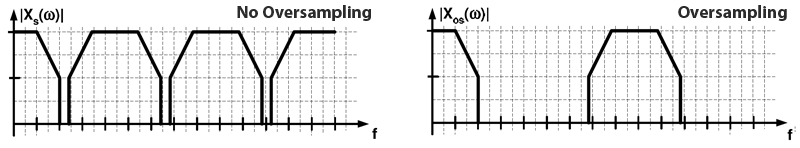
\includegraphics[width=10cm]{../NaT1/bilder/dig_oversampling.png}
	\end{center}

\subsubsection{Natural Sampling\formelbuch{111-5.9}}
Signal mit Periodendauer $T_S$ wird für die Zeit $d$ geschlossen. Amplitude ist bleibt
während Sample nicht konstant. \\
%TODO : Checkliste berechnung des Spektrums für beliebiges Signal

	\begin{center}
		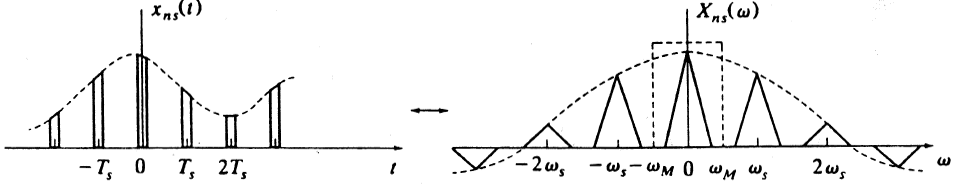
\includegraphics[width=10cm]{../NaT1/bilder/dig_naturalsampling.png}
	\end{center}

\subsubsection{Flat-Top Sampling - Sample \& Hold\formelbuch{112-5.10}}
Das Sample hat die Breite $d$ und bleibt über diese Zeit konstant. \\
Anwendungsbeispiel: A/D-Wandler, Sample \& Hold Schaltung. \\
%TODO : Checkliste berechnung des Spektrums für beliebiges Signal
	\begin{center}
		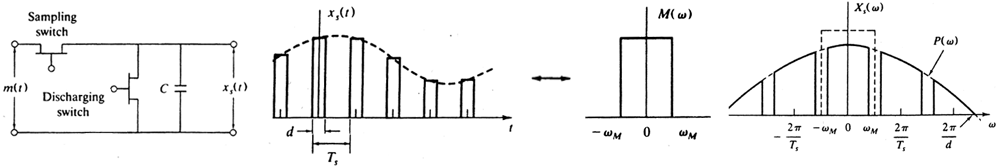
\includegraphics[width=17.5cm]{../NaT1/bilder/dig_flattopsampling.png}
	\end{center}
Das Spektrum des gesampelten Signals wird bei \textbf{höheren Frequenzen} gedämpft, dieses Phänomen
wird als \textbf{Aperture Effect} bezeichnet. Dies kann mit entsprechenden Filtern wieder
korrigiert werden.\\
\hrule
 
\subsection{Quantisierung (Quantizing)\formelbuch{93-5.6}}
	\begin{center}	
		\textbf{Gleichförmig} \hspace{3cm}
		\textbf{Kompressor} \hspace{2.9cm}
		\textbf{$\mu$-Law} \hspace{3cm}
		\textbf{A-Law}  \\
		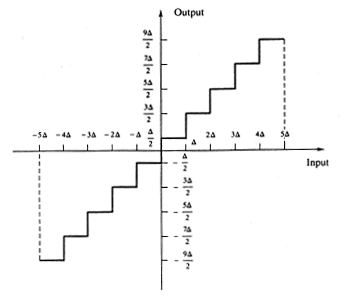
\includegraphics[height=4cm]{../NaT1/bilder/dig_quant_gleichfoermig.png} \hspace{0.5cm}
		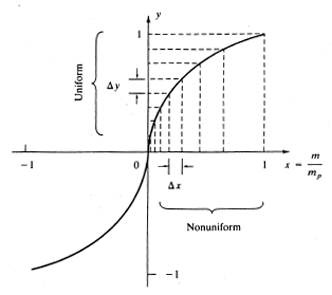
\includegraphics[height=4cm]{../NaT1/bilder/dig_quant_ungleichfoermig.png} \hspace{0.5cm}
		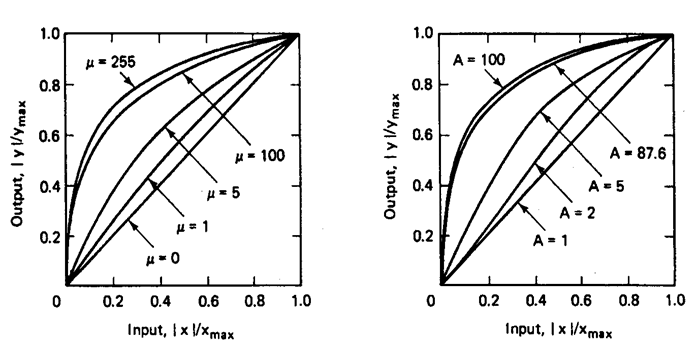
\includegraphics[height=4cm]{../NaT1/bilder/dig_quant_lulaw_ralaw.png}	
	\end{center}
	$\mu$-Law und A-Law sind vor allem bei Signalen mit niedrigem Crest-Faktor von Vorteil: $C = \frac{|x|_{pk}}{x_{RMS}}$

\skriptsubsubsection{Gleichförmige(Uniform) Quantisierung}{93-5.4A}
\begin{minipage}{9cm}
	$$ \Delta = \frac{A_m}{2^{n-1}} = \frac{2 \cdot A_m}{L} \qquad \qquad L = 2^n$$ 
	$$ - \frac{\Delta}{2} \leq q_e \leq \frac{\Delta}{2} \qquad \qquad <q_e^2> = \frac{\Delta^2}{12} =
	\frac{(2 A_m)^2}{L^2 \cdot 12}$$ \vspace{0.1cm}
	$$ \text{SNR} =\frac{S}{N_q}= \frac{S}{q_e^2}$$\\
	$$\text{SNR}_{dB}=10 \log(\text{SNR}) \cdot dB \approx n \cdot 6dB$$
\end{minipage}
\begin{minipage}{9cm}
	$\Delta$ Intervallbreite \\
	$L$ Anzahl Intervalle \\
	$n$ Wortlänge der Samples, [Anzahl Bit] \\
	$A_m$ Amplitude des Nachrichtensignals \\
	$q_e$ Quantisierungsfehler \\
	$<q_e^2>$ Quantisierungsrauschen \\
	SNR Signal-Geräusch Abstand, $[\text{SNR}] = dB$
\end{minipage}


\skriptsubsubsection{Ungleichförmige(Nonuniform) Quantisierung}{95-9.5C}
Bei tiefen Nutzsignalen hat die gleichförmige Quantisierung den Nachteil einer schlechten SNR
(Signal - Geräusch Abstand). \\
Beihilfe schafft die Ungleichförmige Quantisierung z.B. bei Telefonie
A-Law-(Europa) oder $\mu$-Law-Codierung (USA, Japan)). \\
Praktisch wird dies mit einem sogenannten \textbf{Kompressor} und einem nachgeschalteten
gleichförmigen Quantisierer realsiert.

\begin{minipage}{9cm}
$$ f_{\mu-Law}(x) = \sgn(x) \frac{\ln(1+\mu\cdot|x|)}{\ln(1+\mu)}$$
$$\text{SNR}_{\mu-Law} \approx 10 \log \dfrac{3 L^2}{[\ln(1 + \mu)]^2}$$
\end{minipage}
\begin{minipage}{9cm}
$$f_{A-Law}(x)=\begin{cases} \frac{A}{1+ \ln A} x & \mbox{wenn }0 \le x \le \frac{1}{A} \\
	\frac{1}{1+ \ln A} + \frac{\ln Ax}{1+ \ln A}, & \mbox{wenn } \frac{1}{A} < x \le 1 \end{cases} $$
$$\text{SNR}_{A-Law} \approx 10 \log \dfrac{3 L^2}{(1+\ln A)^2}$$
\end{minipage}
\hrule

\skriptsubsection{Codierung (Encoding)}{96-5.7}

\skriptsubsubsection{Bandbreitenbedarf von PCM-Signalen}{96-5.8}
\begin{minipage}{9cm}
	$$ f_s > 2 \cdot B_m  \qquad \qquad n = \log_2 L$$ 
	$$ R_B = f_s \cdot n > 2 \cdot n \cdot B_m $$ 
	$$ B_{eff} > B_{PCM} = \frac{1}{2} n \cdot f_s > n \cdot B_m$$
\end{minipage}
\begin{minipage}{9cm}
	$f_s$ Samplingrate, $[f_s] = Hz$ \\
	$n$ Bits pro Sample, \textcolor{red}{ganzzahlig} \\
	$R_B$ Bitrate des PCM-Signals, $[R_B] = \frac{bit}{s}$ \\
	$B_m$ Signalbandbreite, $[B_m] = Hz $ \\
	$B_{PCM}$ Bandbreite PCM Signal, $[B_{PCM}] = Hz $
\end{minipage}


\skriptsubsubsection{Delta Modulation}{97-5.9}
\begin{minipage}{9cm}
$$ \frac{\Delta}{T_s} = \Delta \cdot f_s > \left| \frac{d m(t)}{dt} \right|_{max}$$
$$ (\text{SNR})_0 = 10 \cdot \log\left(\frac{3 f_s^3}{8 \pi^2 f_m^2 f_M}\right) \cdot dB$$ 
$$ <q_e^2> = \frac{\Delta^2}{3} $$ 
\end{minipage}
\begin{minipage}{9cm}
	$f_s$ Samplingrate, $[f_s] = Hz$ \\
	$f_m$ Signalfrequenz, $[f_m] = Hz$ \\
	$f_M$ Grenzfrequenz des TP-Filters, $[f_M] = Hz$ \\
	$B_m$ Signalbandbreite, $[B_m] = Hz $ \\
	$B_{PCM}$ Bandbreite PCM Signal, $[B_{PCM}] = Hz $\\
	$\Delta$ Schritthöhe\\
	$<q_e^2>$ Quantisierungsrauschen \\
	
\end{minipage}

\skriptsubsubsection{Leitungscodierung}{99-5.10}
Je nach Anforderungen (DC-Freie Übertragung, Clock-Rückgewinnung, Störfestigkeit,
Bandbreitenbedarf, Erkennung von Übertragungsfehlern) wird das zu übertragende Signal entsprechend
codiert.

\begin{minipage}{9cm}
	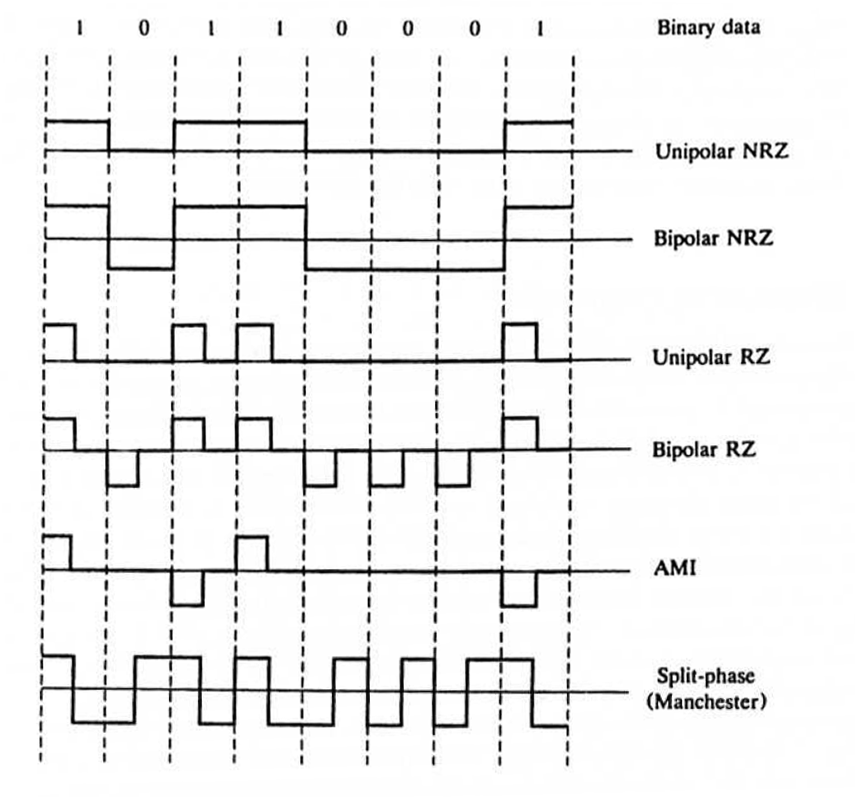
\includegraphics[width=8.7cm]{../NaT1/bilder/dig_leitungscodierung.png}
\end{minipage}
\begin{minipage}{9cm}
	\textbf{Unipolar NRZ(Nonreturn-to-Zero)} \\
	1 = Puls, 0 = kein Puls \\ \\
	\textbf{Bipolar NRZ(Nonreturn-to-Zero)} \\
	1 = positiver Puls, 0 = negativer Puls \\ \\
	\textbf{Unipolar (RZ)Return-to-Zero} \\
	1 = Puls der wieder auf Null zurückspringt, 0 = kein Puls \\ \\
	\textbf{Bipolar RZ} \\
	1 = positiver Puls (kehrt wieder auf Null zurück), 0 = negativer Puls (kehrt wieder auf Null
	zurück)\\ \\
	\textbf{AMI (Alternate Mark Inversion) RZ} \\
	1 = Abwechslungsweise positiver und negatier Puls, 0 = kein Puls. DC-frei\\ \\
	\textbf{Split-Phase (Manchester)} \\
	1 = Positiver Puls mit anschliessend Negativem, 0 = Negativer Puls mit anschliessendem Positivem. DC-frei, einfache Synchronisation
\end{minipage}


\skriptsubsubsection{Pulse Shaping und ISI (Intersymbolic Interference)}{101-5.13A}
Da Übertragungskanäle in der Praxis keine idealen Eigenschaften 
(\textbf{limitierte Bandbreite}, Nichtlinearität, Verzerrungen) aufweisen,
werden die - von uns als rechteckig
angenommenen - Pulse verfälscht. Die Pulse werden \textbf{verbreitert} und \textbf{überlappen}
benachbarte Pulse, sodass beim Empfänger eine Unterscheidung der verschiedenen Symbole schwer
fällt. \\
Das oben erwähnte Phänomen wird \textbf{intersymbolic interference} genannt. \\
Abhilfe schafft ein passendes Filter, welches dem Übertragungskanal vorgeschaltet wird. Das Filter
weist eine spezielle Impulsantwort auf, welche bei \textbf{gleichmässigen Zeitabständen}
(Abtastzeiten) Null ist, ausser zum Zeitpunkt Null. Dadurch kann die ISI umgangen werden, wenn dann
genau zu diesen Zeiten abgetastet wird. \\ 

\textbf{Raised-Cosine Filter \formelbuch{103}} \\
Dieses Filter schafft Abhilfe bei ISI. Obwohl dies auch mit einem Idealen Filter
(Sinc-Frequenzgang) möglich wäre, wird ein Raised-Cosine mit folgenden Vorteilen eingesetzt:
\begin{itemize}
  \item Raised-Cosine-Puls fällt schneller ab als Sinc-Puls
  \item Raised-Cosine ist zwar auch akausal, aber in der Praxis einfacher realisierbar 
\end{itemize}

\begin{minipage}{9cm}
$$ f_B = \frac{1 + \alpha}{2 T} Hz \qquad \qquad \frac{1}{T} = \frac{2 f_B}{1 + \alpha}$$
\end{minipage}
\begin{minipage}{9cm}
	$f_B$ benötigte Bandbreite, $[f_B] = Hz$ \\
	$\frac{1}{T}$ Pulsrate, $[\frac{1}{T}] = $ "Pulse pro Sekunde" \\
	$\alpha$ roll-off-Faktor, $[\alpha] = 1$ 
\end{minipage}

\begin{center}  
		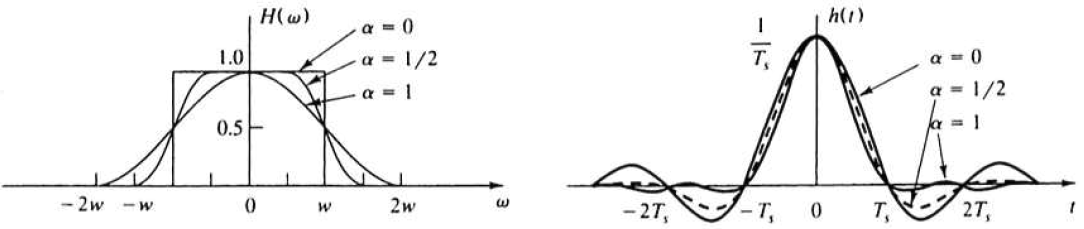
\includegraphics[height=3.2cm]{../NaT1/bilder/dig_raisedcosinefilter.png}
\end{center}


$$ 
h(t) = \frac{1}{T_s} = \left( \frac{\sin{W t}}{W t} \right) \left[ \frac{\cos{\alpha W t}}{1
- (2 \alpha W t / \pi)^2}\right]
\quad \laplace \quad
H(\omega) = \begin{cases}
	1 			
		&  	0 \leq | \omega | \leq (1-\alpha) W       \\
	\frac{1}{2} \left( 1 - \sin\left[ \frac{\pi}{2 \alpha W} (| \omega | - W)\right] \right)      
		&	(1-\alpha) W \leq | \omega | \leq (1+\alpha) W       \\
	0
		& 	| \omega | > (1+\alpha) W
            \end{cases}
$$


% 
% Vorteil Raised-Cosine zu Sinc: RCosine fällt schneller ab (wenn t gegen unendlich). \\
% RCosine ist zwar auch akausal aber kann viel besser approximiert(praktisch realisiert) werden als
% ein sinc, da er schneller abfällt!

\skriptsubsubsection{Digitale Trägermodulation}{104-5.14}
\begin{minipage}{9cm}
	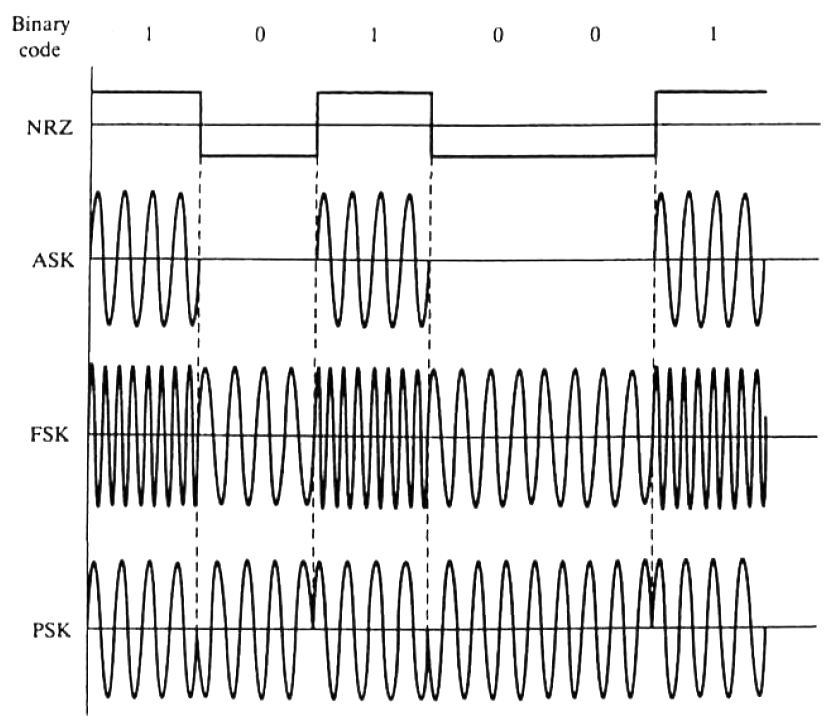
\includegraphics[width=8.7cm]{../NaT1/bilder/dig_traegermodulation.png}
\end{minipage}
\begin{minipage}{9cm}
	Weil Binäre Nachrichtensignale selbst zu kleine Frequenzen aufweisen, sind sie nicht geeignet um
	z.B. über den Äther zu schicken. Abhilfe schafft die binäre Trägermodulation. 
	\vspace{1cm}  \\
	\textbf{ASK - Amplitude-Shift Keying} \\
	$$x_c(t) = \begin{cases}
           A \cos(\omega_c t) & \textbf{symbol 1} \\
           0 & \textbf{symbol 0}
           \end{cases} $$ \\
	\textbf{FSK - Frequency-Shift Keying} \\
	$$x_c(t) = \begin{cases}
           A \cos(\omega_{c1} t) & \textbf{symbol 1}     \\         
           A \cos(\omega_{c2} t) & \textbf{symbol 0}
           \end{cases} $$ \\
	\textbf{PSK - Phase-Shift Keying} \\
	$$x_c(t) = \begin{cases}
           A \cos(\omega_{c} t) & \textbf{symbol 1}        \\      
           A \cos(\omega_{c} t + \pi) & \textbf{symbol 0}
           \end{cases} $$ \\
\end{minipage}